\subsection{什么是圆锥曲线}

\begin{definition}
    圆锥曲线是通过平切圆锥（严格为一个正圆锥面和一个平面完整相切）得到的曲线，包括椭圆，抛物线，双曲线及其他一些退化类型。
\end{definition}

下面是圆锥曲线的分类：

\begin{figure} [H]
    \centering
    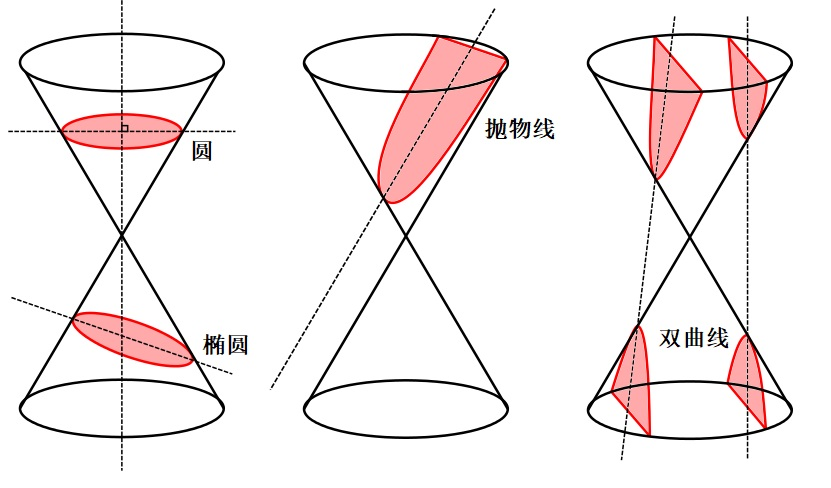
\includegraphics[width=0.45\textwidth]{chapters/圆锥曲线/images/圆锥曲线引入/img-20250728131909.png}
    \caption{被斜切得到的三种曲线}
\end{figure}

\subsection{求曲线的交点}

\begin{theorem}
    \begin{multicols}{2}
        在求直线和直线的交点时，我们将两条直线联立了起来：
        $$
            \begin{cases}
                A_1x + B_1y + C_1 = 0 \\
                A_2x + B_2y + C_2 = 0
            \end{cases}
        $$

        \columnbreak

        求曲线的交点时也是一样的做法：
        $$
            \begin{cases}
                f_1(x,y) = 0 \\
                f_2(x,y) = 0
            \end{cases}
        $$
    \end{multicols}
\end{theorem}

\begin{example}
    曲线 $x^2+x y-y-3=0$ 与直线 $y=x$ 交于 $A $、$B$ 两点，则线段 $A B$ 的长度为 \underline{\qquad}.
\end{example}

\vspace{8em}

\subsection{求轨迹方程}

\subsubsection{直译法}

\begin{definition}
    轨迹问题最重要的是根据题目要求，根据定义或题目中已知的条件关系，列出对应的方程。
\end{definition}

\begin{theorem}
    常用到的有：

    \begin{enumerate}
        \item 斜率构造：已知 $A(x_1,y_1), B(x_2,y_2), P(x,y)$，且 $k_{PA} \cdot k_{PB} = C$，其中 $C$ 为常数。
        \item 两点间距离公式：$\sqrt{(x_1-x_2)^2 + (y_1-y_2)^2}$
        \item 斜率之积、斜率之和等。
    \end{enumerate}
\end{theorem}

\begin{example}
    点 $M$ 与定点 $F(2,0)$ 的距离和它到定直线 $x=8$ 的距离之比为 $1: 2$ ，则 $M$ 的轨迹方程是

    \begin{tasks}(4)
        \task $y^2=8 x$
        \task $y^2=-8(x-4)$
        \task $\frac{x^2}{4}-\frac{y^2}{3}=1$
        \task $\frac{x^2}{16}+\frac{y^2}{12}=1$
    \end{tasks}
\end{example}

\v{8em}

\begin{example}
    动点 $P(x, y)$ 到两定点 $A(-3,0)$ 和 $B(3,0)$ 的距离的比等于 2 ，求动点 $P$ 的轨迹方程．
\end{example}

\begin{theorem}[阿氏圆]
    设点 $P$ 在平面内运动，$A, B$ 是平面内的两定点，满足 $\frac{|PA|}{|PB|} = k$，则点 $P$ 的轨迹是一个圆。
\end{theorem}

\v{8em}

\subsubsection{相关点法}

\begin{example}
    点 $P$ 在椭圆 $\frac{x^2}{9} + \frac{y^2}{5} = 1$ 上运动，设 $O$ 为坐标原点，则线段 $OP$ 的中点 $M$ 的轨迹方程是
    \begin{tasks}(4)
        \task $\frac{x^2}{9/4} + \frac{y^2}{5/4} = 1$
        \task $\frac{x^2}{9/2} + \frac{y^2}{5/2} = 1$
        \task $\frac{x^2}{36} + \frac{y^2}{20} = 1$
        \task $\frac{x^2}{9} + \frac{y^2}{5} = 4$
    \end{tasks}
\end{example}
\begin{solution}
    设点 $P$ 的坐标为 $(x_0, y_0)$，满足 $\frac{x_0^2}{9} + \frac{y_0^2}{5} = 1$。动点 $M$ 的坐标为 $(x, y)$。

    根据中点坐标公式，可得：
    $x = \frac{x_0+0}{2} = \frac{x_0}{2}$
    $y = \frac{y_0+0}{2} = \frac{y_0}{2}$

    从上述关系中，我们可以表示出 $x_0$ 和 $y_0$ 与 $x, y$ 的关系：$x_0 = 2x$, $y_0 = 2y$

    将 $x_0 = 2x$ 和 $y_0 = 2y$ 代入点 $P$ 所满足的椭圆方程 $\frac{x_0^2}{9} + \frac{y_0^2}{5} = 1$ 中，得到点 $M$ 的坐标 $(x,y)$ 所满足的方程：
    $$\frac{(2x)^2}{9} + \frac{(2y)^2}{5} = 1$$
    整理，得到点 $M$ 的轨迹方程：
    $\frac{x^2}{9/4} + \frac{y^2}{5/4} = 1$
\end{solution}

\vspace{2em}

\begin{example}
    若 $Q$ 是 $x^2-y^2=2$ 上任一点，$F$ 是右焦点，点 $P$ 在 $F Q$ 的延长线上，且 $\overrightarrow{P Q}=2 \overrightarrow{Q F}$ ，则 $P$ 点的轨迹方程是 \underline{\qquad}．
\end{example}

\begin{solution}
    设 $Q\left(x_0, y_0\right), P(x, y)$ 由题意可知 $F(2,0)$
    $\because \overrightarrow{P Q}=2 \overrightarrow{Q F}, \therefore\left(x_0-x, y_0-y\right)=2\left(2-x_0,-y_0\right)$.

    \vspace{0.2cm}

    $\therefore\left\{\begin{array}{l}x_0-x=4-2 x_0 \\ y_0-y=-2 y_0\end{array}, \therefore\left\{\begin{array}{l}x_0=\frac{4+x}{3} \\ y_0=\frac{y}{3}\end{array}\right.\right.$ ．又点 $Q$ 在双曲线上，$\therefore x_0^2-y_0^2=2$

    \begin{center}
        $\therefore\left(\frac{4+x}{3}\right)^2-\left(\frac{y}{3}\right)^2=2$ ，整理得 $(x+4)^2-y^2=18$
    \end{center}
\end{solution}

\begin{example}
    椭圆 $C$ 的方程为 $\frac{x^2}{16} + \frac{y^2}{4} = 1$。点 $A$ 为椭圆上任意一点，$Q(2, 1)$ 为定点。求线段 $AQ$ 中点 $N$ 的轨迹方程。
\end{example}

\vspace{8em}

\subsection{求特殊曲线}

\begin{example}
    已知星形线：$C: x^{\frac{2}{3}}+y^{\frac{2}{3}}=8^{\frac{2}{3}}=4$ ，下列说法正确的是 （\qquad）
    \begin{tasks}(3)
        \task 点 $(1,5)$ 在曲线外
        \task 曲线围成的面积小于 128
        \task 直线 $x+y-4 \sqrt{3}=0$ 与曲线有三个交点
    \end{tasks}

    \begin{figure} [H]
        \centering
        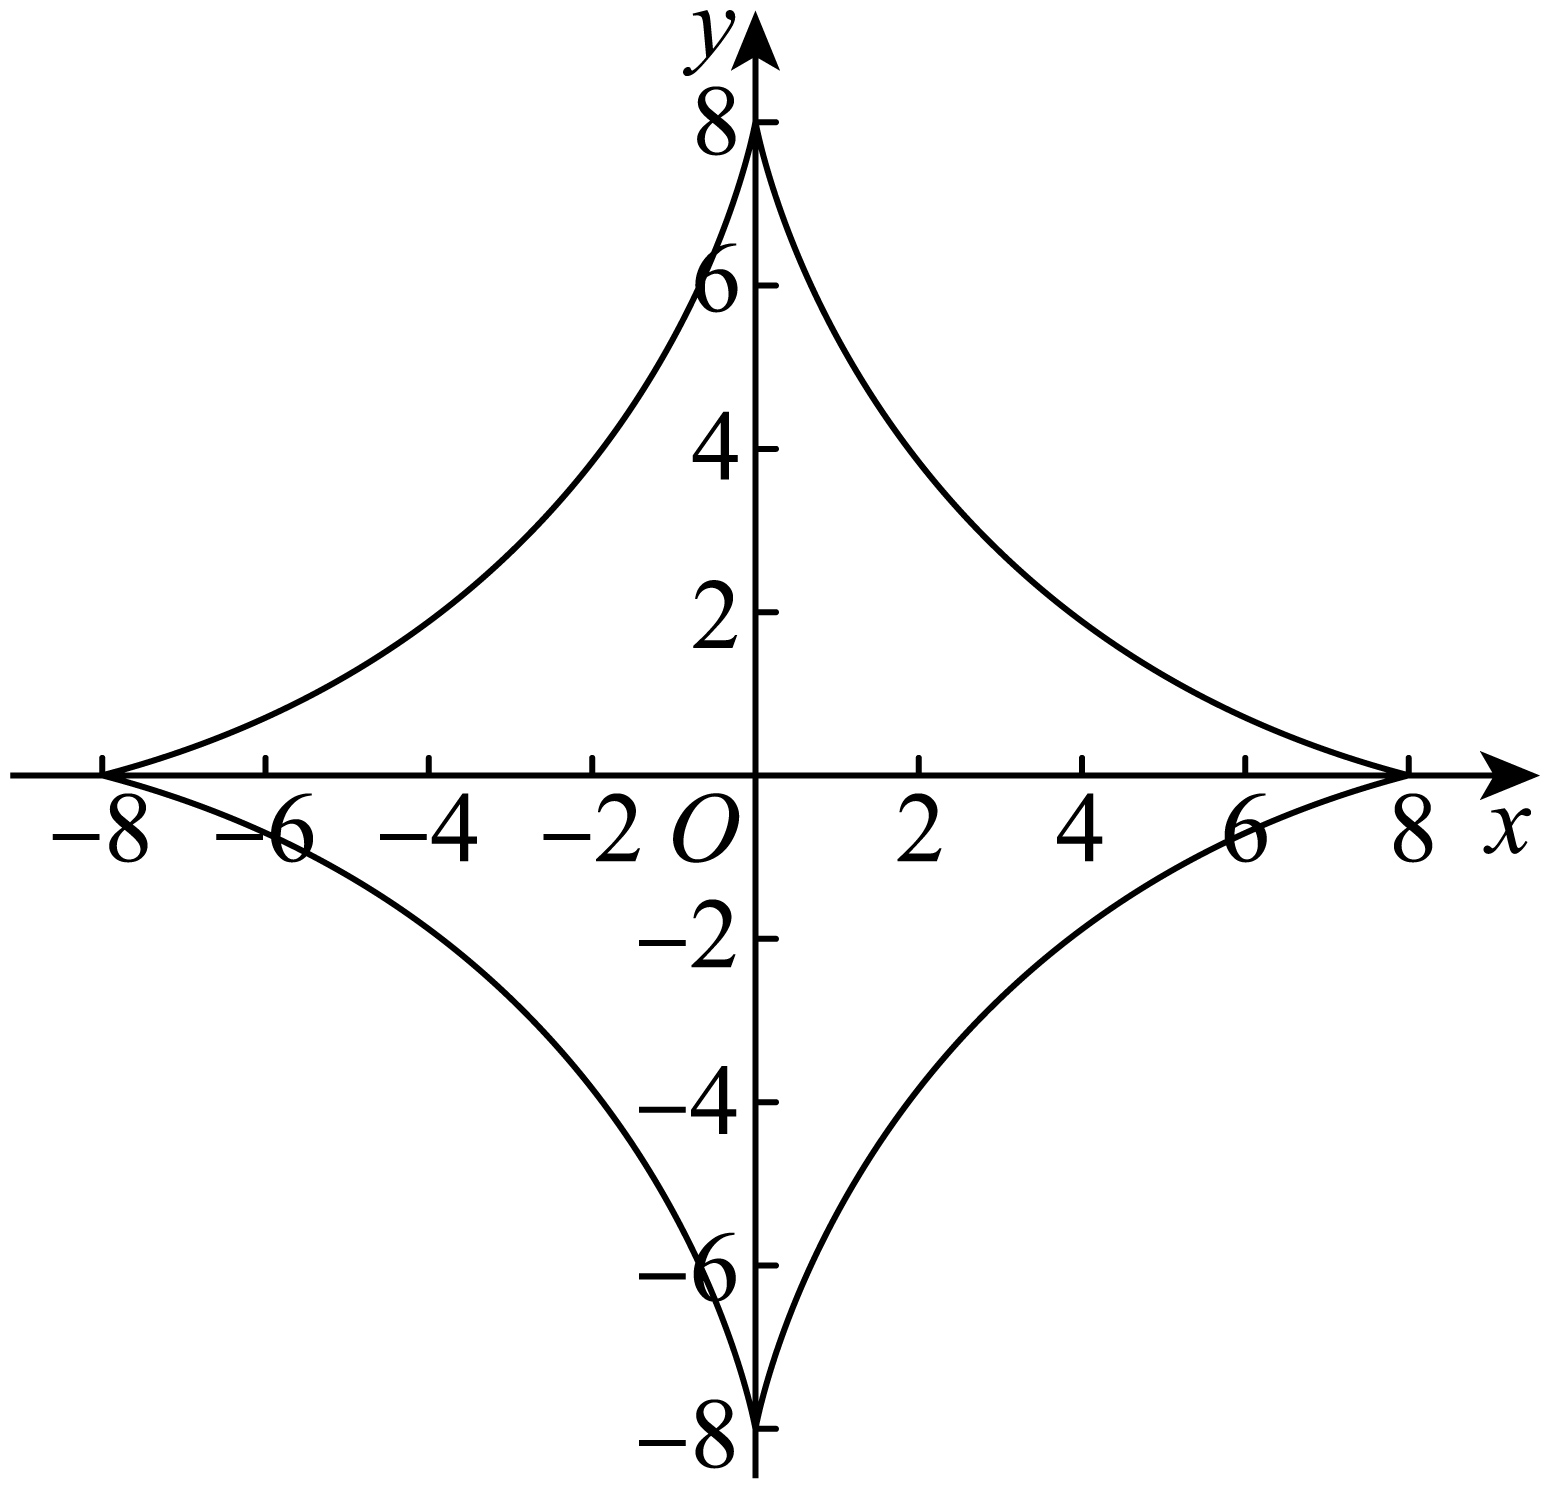
\includegraphics[width=0.2\textwidth]{chapters/圆锥曲线/images/圆锥曲线引入/img-20250728143547.png}
    \end{figure}
\end{example}


